\chapter{Simulation Framework}
The methods described in Chapter \ref{ch:pp} on Path Planning were implemented within a simulation environment in \textit{MATLAB} in order to show the effectiveness of the introduced path planners. The target fields in the simulations are of a variable size with a single state of interest that can be sampled. The autocorrelation factor of the field in the simulation is an adjustable variable that determines the likeliness of each pair of neighboring points as a function of distance. 

\section{Simulated Exploration Vehicle Model Dynamics}
The dynamics of the simulated vehicle are modeled after the vehicle model described in Equation \ref{eq:vehicledynamicsmodel}. In the simulation, $\Delta T$ and $V$ are constants predefined in the simulation environment. For a given waypoint destination, the vehicle will pass over every vesicle on the line connecting its original position and its final position. The vehicle's heading angle and speed can be controlled at any point in the simulation. The path planner directly feeds a control heading angle to the simulated vehicle. The speed of the vehicle is kept constant. A trajectory (a set of waypoints), $T$, calculated in Chapter \ref{ch:pp}, is loaded into a waypoint queue for the vehicle, where each waypoint is met one after another. After meeting the final waypoint in the trajectory, the next set of waypoints is calculated by a path planner. The process continues until the termination condition (maximum area scanned) is satisfied. A sample is taken at every possible vesicle that the vehicle passes over. The location and value of each sample is stored in the vehicle object's memory for later use in the prediction procedures.

% The dynamics of the simulated exploration vehicle are modeled off of a Dubins' Vehicle with a variable turning radius, $r$. The simulated vehicle has constant vehicle velocity of $V$, and a heading angle, $\theta$.

% \begin{equation}
% \dot{\vect{X}} =
% 	\begin{bmatrix}
% 		\dot{x_1} \\
% 		\dot{x_2} \\
% 		\dot{\theta} \\
% 	\end{bmatrix} = 
% 	\begin{bmatrix}
% 		V \cos \theta \\
% 		V \sin \theta \\
% 		\omega
% 	\end{bmatrix}
% \end{equation}

% Where $\dot{\vect{X}}$ is the time derivative of the vehicle's state vector, and $\omega$ is the vehicle's turn rate control. The vehicle's state vector is discretized as $\vect{X}_{k+1}$.

% \begin{equation}
% \vect{X}_{k+1} = \vect{X}_k +
% 	\begin{bmatrix}
% 		V \Delta T \cos \theta_k \\
% 		V \Delta T \sin \theta_k \\
% 		\omega_k
% 	\end{bmatrix}
% \end{equation}
% 
% Where $\Delta T$ and $V$ are constants predefined in the simulation environment. For a given waypoint destination, a Dubin's path is calculated for the vehicle. A control angular velocity for each time step, $\omega_k$, is calculated for the trajectory. A trajectory (a set of waypoints), $T$, calculated in Chapter \ref{ch:pp}, is loaded into the Dubin's path trajectory finder for the vehicle from the current position of the vehicle to the first waypoint in the trajectory. After meeting the waypoint, the next path to the next waypoint is calculated. This process continues up to the last waypoint in the trajectory set, $T$. A new trajectory is then calculated by the path planner, and the process continues until the termination condition is satisfied.
% \subsection{Caveats of Result Simulation}
% The simulated exploration vehicle will take on the dynamics of a vehicle with a very small radius of turn (ROT) ($r = 10^{-4}$). The ROT is made small to show the effectiveness of the path planners on their own, independent of the exploration vehicle's dynamics. The velocity of the vehicle is set to move a single unit of distance on the field per sample period. Furthermore, the target field in the simulation is fully-ergodic, and the speed of flight does not change the quality of prediction.
\section{Generating a Target Field}
The simulation yields a target field that is of variable height $h$, and width $w$. Each vesicle in the field is exactly the area of the sensor footprint of the simulated vehicle's sensor. This is to make the sensor measurements as ideal as possible, so no samples are missed when a vesicle is flown over.

The field is composed of a single feature which is autocorrelated spatially. Initially, the points on the field are generated from a normal distribution with a standard deviation of $1$, and expected value of $0$. The field is then convolved with a two dimensional Gaussian filter, $G(x,y,\sigma_{field})$ (Equation \ref{eq:gauss_filt}), with a variable standard deviation, $\sigma_{field} \in \mathbb{R}_{\geq 0}$ which sets the radius of the filter. 

\begin{equation}
G(x,y,\sigma_{field}) = \frac{1}{2 \pi \sigma_{field}^2} e^{\frac{x^2 + y^2}{2\sigma_{field}^2}}
\label{eq:gauss_filt}
\end{equation}

\noindent where $x \in \mathbb{N}$, $y \in \mathbb{N}$, and for all values $x \in [1, w], y \in [1, h]$.

The Gaussian filter ``smooths" the field in order to simulate autocorrelation. In \textit{MATLAB}, the \textit{imfilter} function is used to perform a 2D convolution on the randomly generated field. The result is a randomly-generated, variably-sized, and autocorrelated field with a unit-less feature of interest. One such field can be observed in Figure \ref{fig:gen_field}. As the value of the standard deviation of the Gaussian filter kernel, $\sigma_{field}$, increases, the field exhibits higher spatial autocorrelation. Inversely, when $\sigma_{field}$ is close to zero, the field becomes has no signs of spatial autocorrelation.

% \begin{figure}[htb!]
% 	\begin{subfigure}
% 		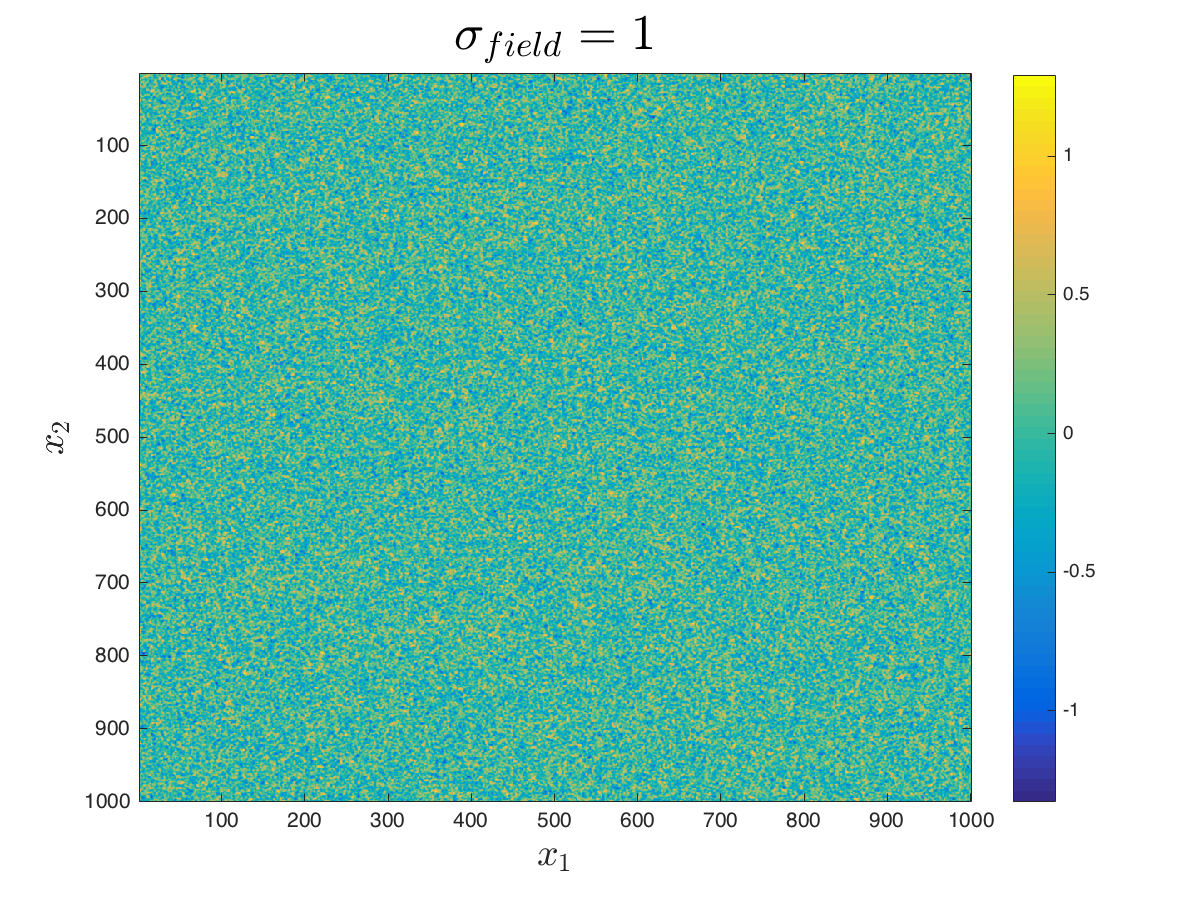
\includegraphics[width=0.45\linewidth]{figures/autocorr_sigma_1.png}
% 		\subcaption{$\sigma_{\text{field}} = 1$. The field apears to exhibit very low spatial autocorrelation.}
% 	\end{subfigure}
% 	~
% 	\begin{subfigure}
% 		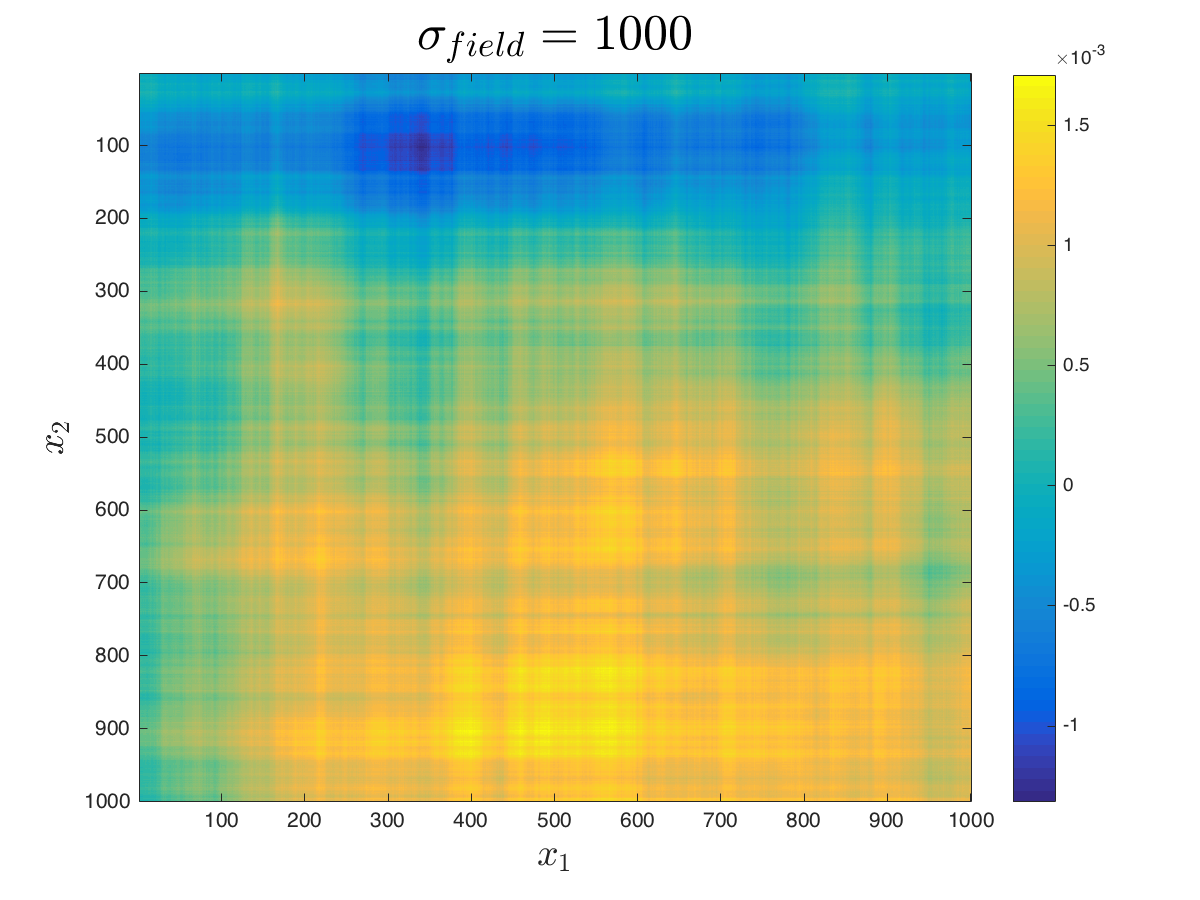
\includegraphics[width=0.45\linewidth]{figures/autocorr_sigma_1000.png}
% 		\subcaption{$\sigma_{\text{field}} = w$, where $w = 1000$ is the field width and height. The field is more spatially autocorrelated.}
% 	\end{subfigure}
% \end{figure}

\begin{figure}[ht!]
    \centering
    \begin{subfigure}[t]{0.33333\textwidth}
        \centering
        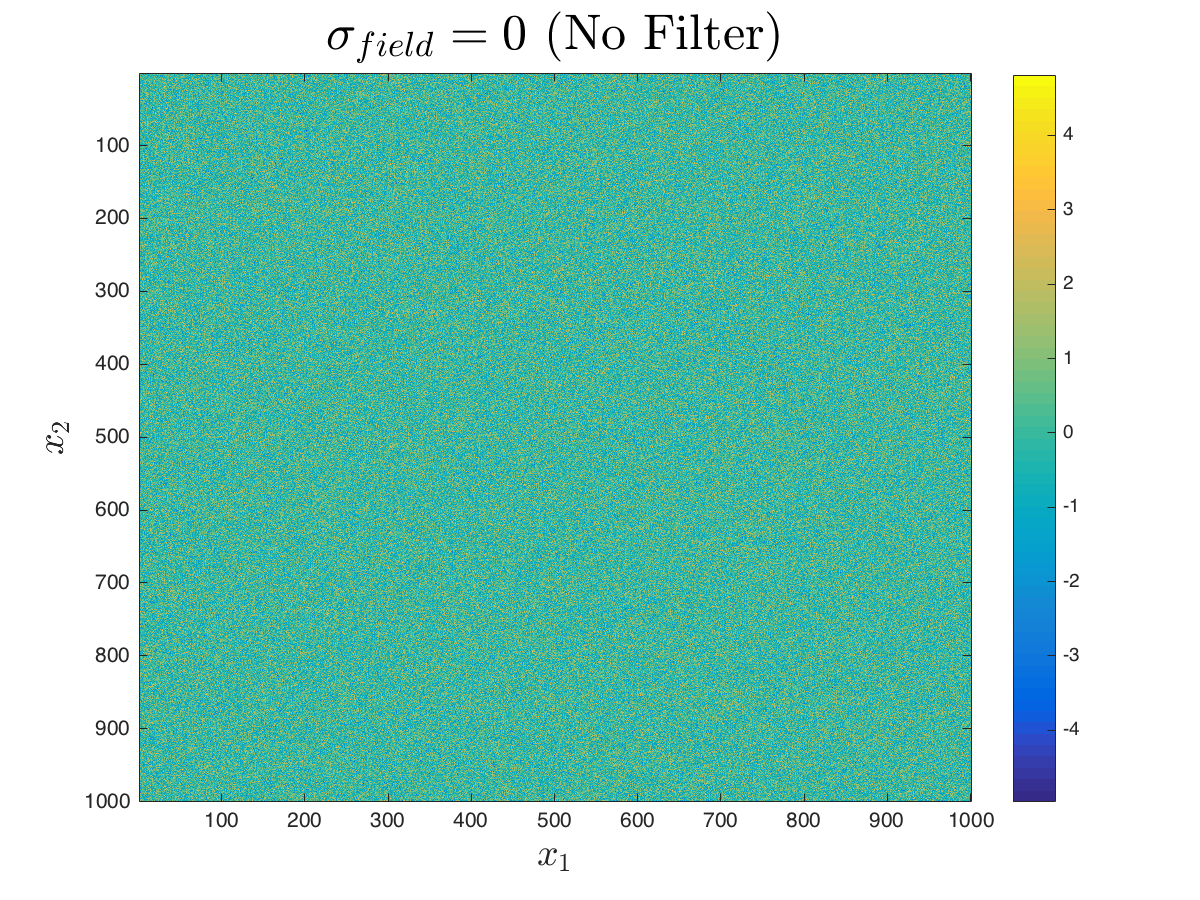
\includegraphics[width=\linewidth]{figures/autocorr_sigma_0.png}
        \captionsetup{skip=0.25\baselineskip,size=footnotesize}
        \ssp
        \caption{$\sigma_{field} = 0$. The field exhibits no spatial autocorrelation.}
    \end{subfigure}%
    ~
    \begin{subfigure}[t]{0.33333\textwidth}
        \centering
        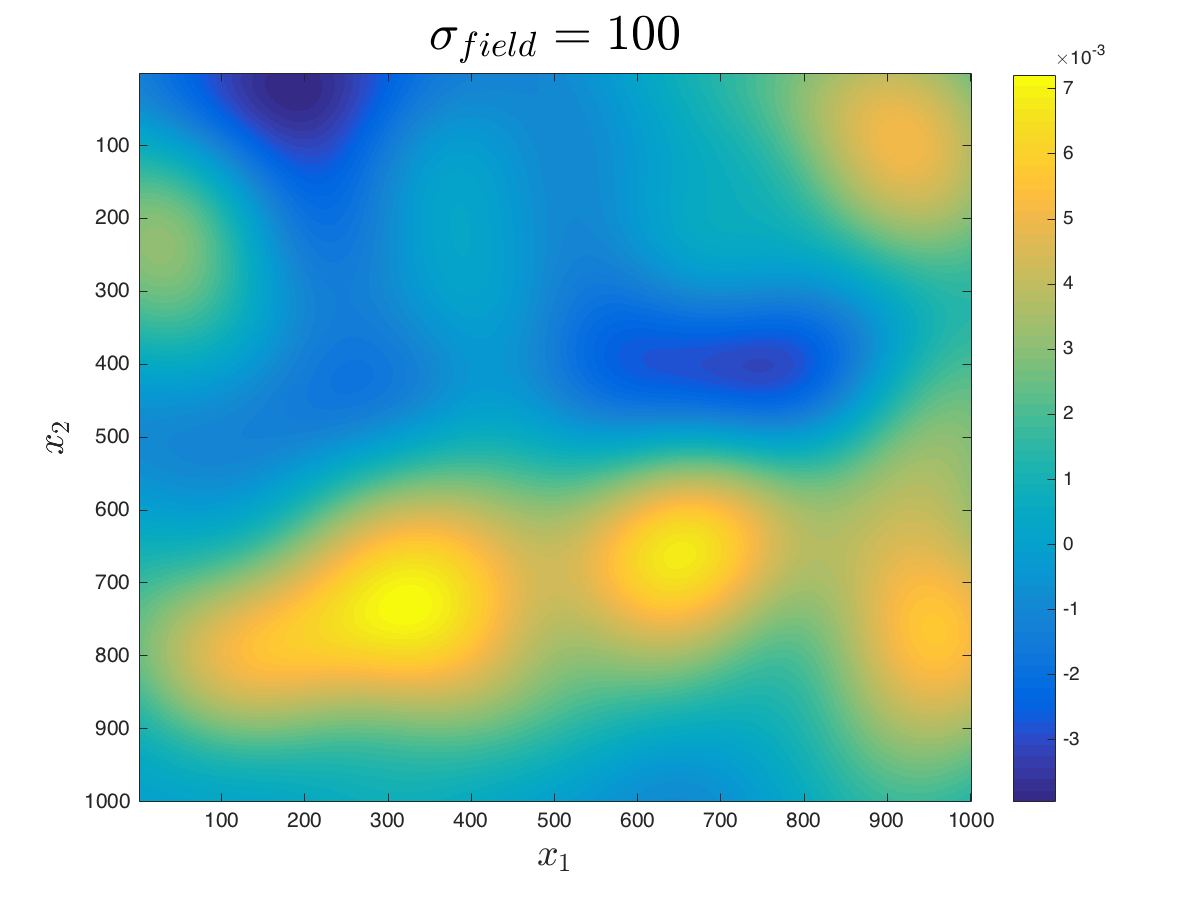
\includegraphics[width=\linewidth]{figures/autocorr_sigma_100.png}
        \captionsetup{skip=0.25\baselineskip,size=footnotesize}
        \ssp
        \caption{$\sigma_{field} = \frac{w}{10} = 100$. The field appears to exhibit some degree of spatial autocorrelation.}
    \end{subfigure}%
    ~ 
    \begin{subfigure}[t]{0.33333\textwidth}
        \centering
        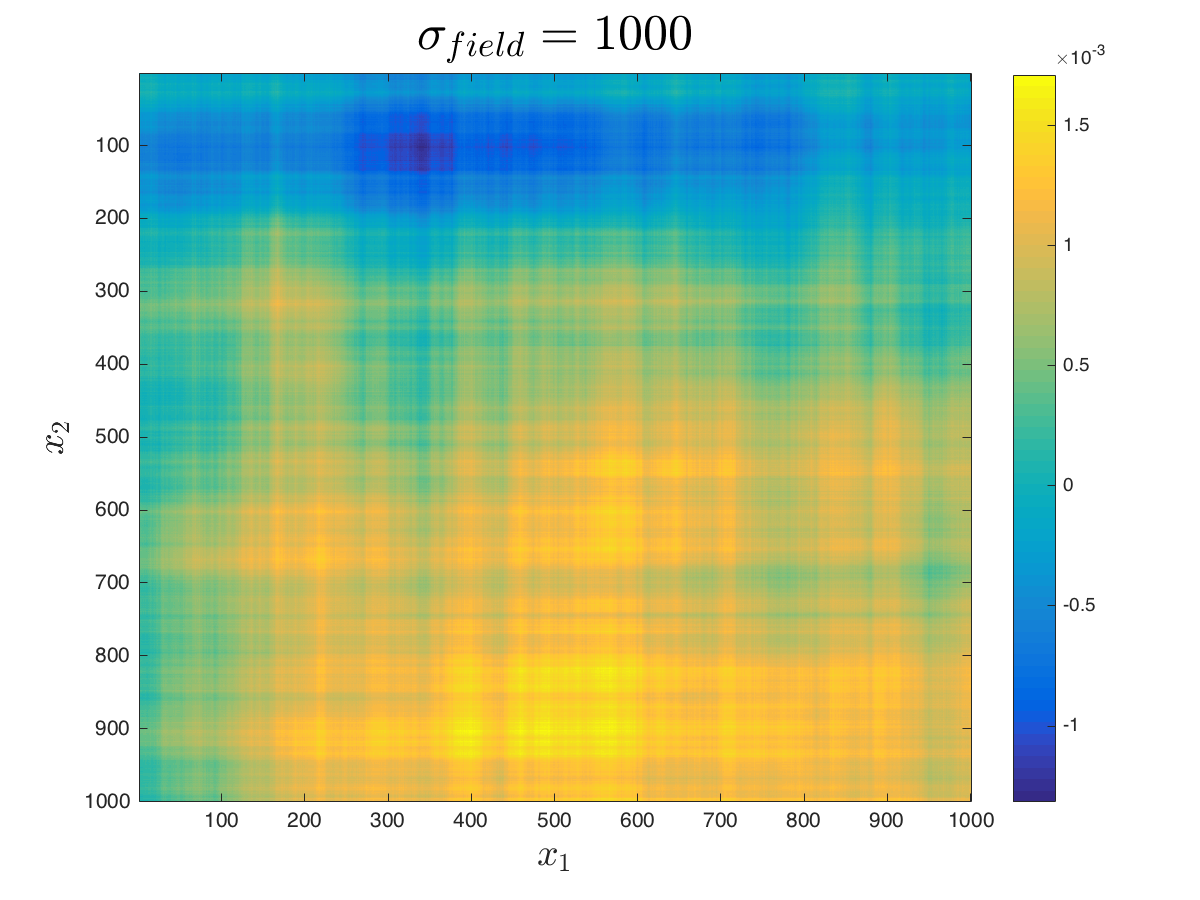
\includegraphics[width=\linewidth]{figures/autocorr_sigma_1000.png}
		\captionsetup{skip=0.25\baselineskip,size=footnotesize}
		\ssp
        \caption{$\sigma_{field} = w = 1000$. The field exhibits a high degree of spatial autocorrelation.}
    \end{subfigure}
    \ssp
    \caption{A field is generated using a random number generator with a zero mean normal distribution with variance $1$. Varying degrees of spatial autocorrelation are shown for different values of $\sigma_{field}$.}
\end{figure}

\section{Simulation Environment}
The simulation, once started, runs a single exploration method at a time starting with the same random number seed. A generated field is initially unknown to a vehicle object, but samples are collected as it passes along the field. The variances of Kriging predictions, the currently predicted field, and the path traversed are plotted along with the actual field being explored.

\begin{figure}[htb!]
    \centering
    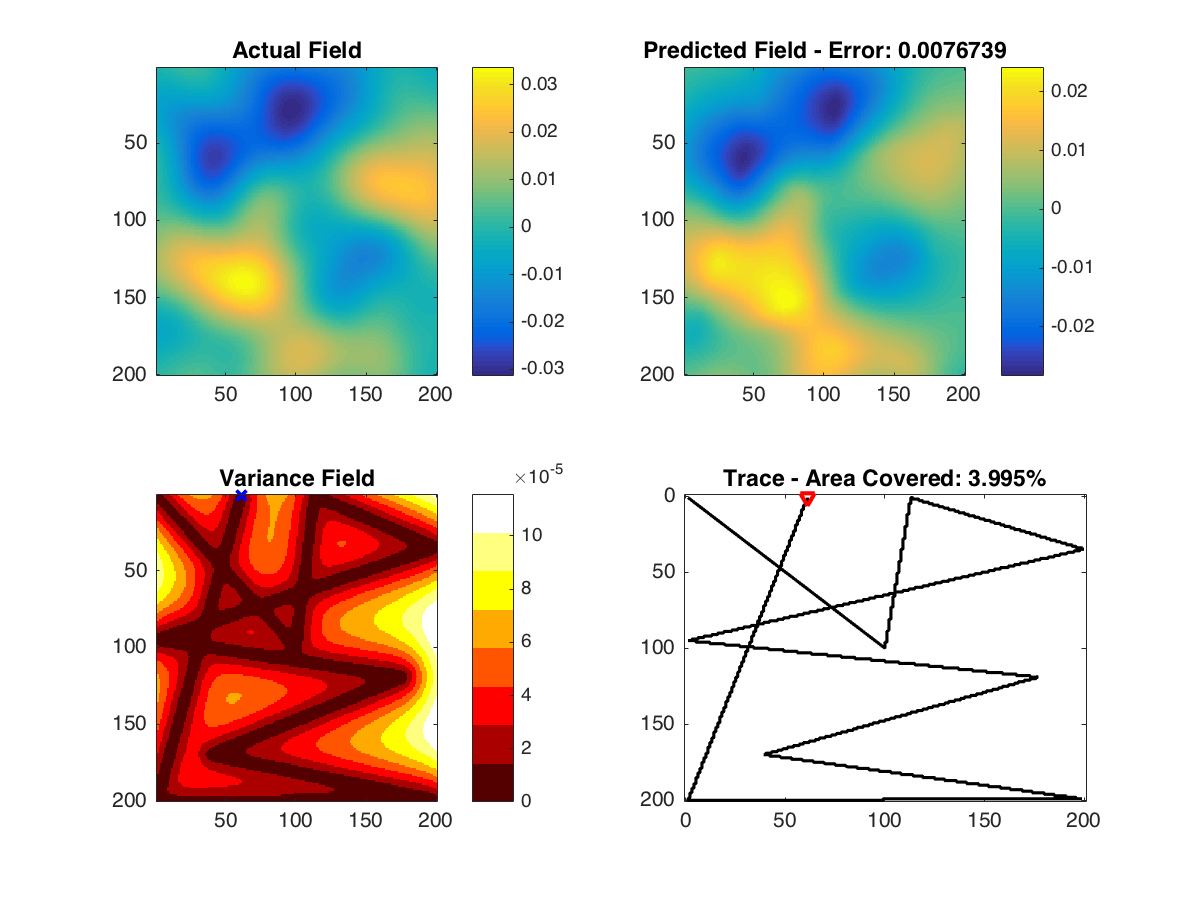
\includegraphics[width=0.8\linewidth]{figures/sim_figures/nhv_3_5p_200x200_sf_20_seed_2}
	\captionsetup{skip=0.25\baselineskip}
	\ssp
    \caption{Highest Variance Path Planning. The actual field (top left), predicted field (with error) (top right), variance field (bottom left), and traversed path (bottom right).}
\end{figure}

\begin{figure}[htb!]
    \centering
    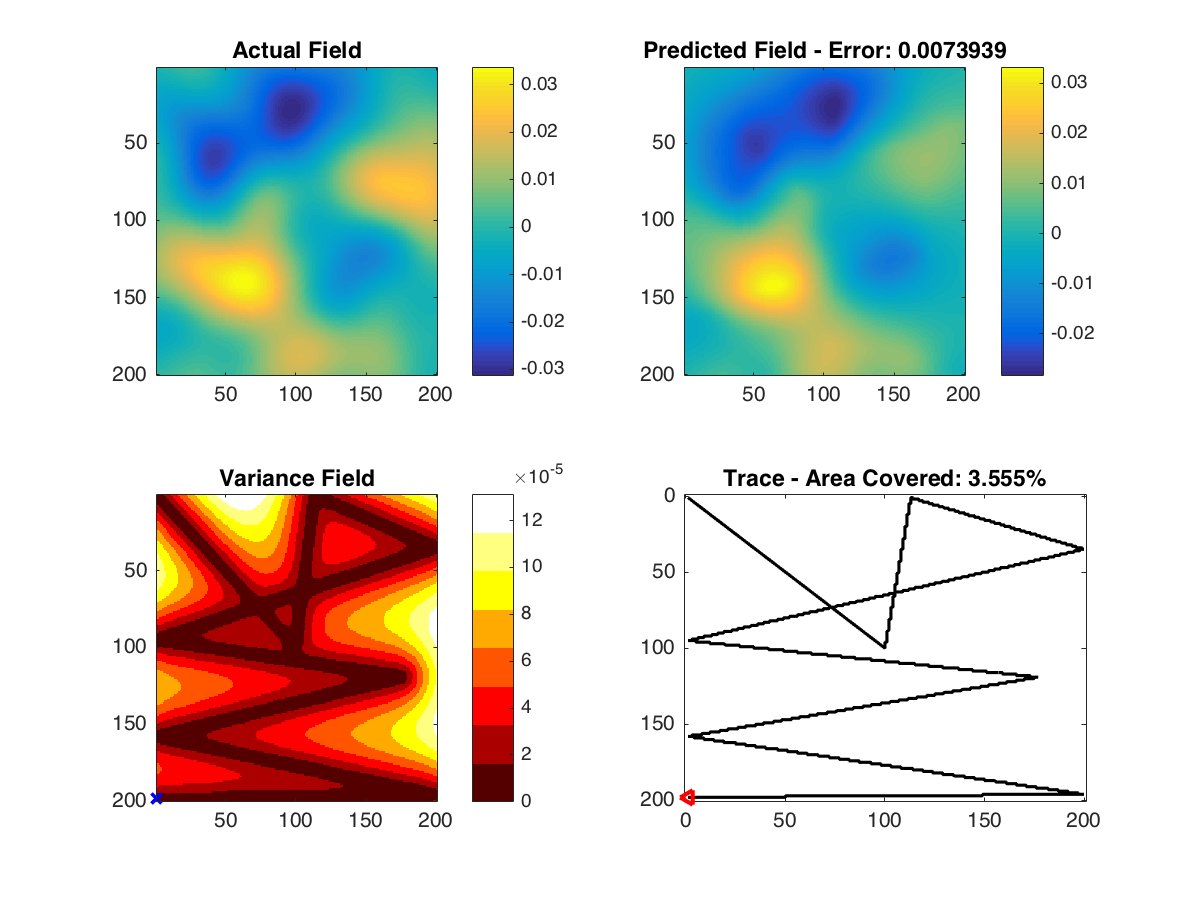
\includegraphics[width=0.8\linewidth]{figures/sim_figures/nnhv_3_5p_200x200_sf_20_seed_2}
    \captionsetup{skip=0.25\baselineskip}
    \ssp
    \caption{$N$ Highest Variance Path Planning ($N=5$). The actual field (top left), predicted field (with error) (top right), variance field (bottom left), and traversed path (bottom right).}
\end{figure}

\begin{figure}[htb!]
    \centering
    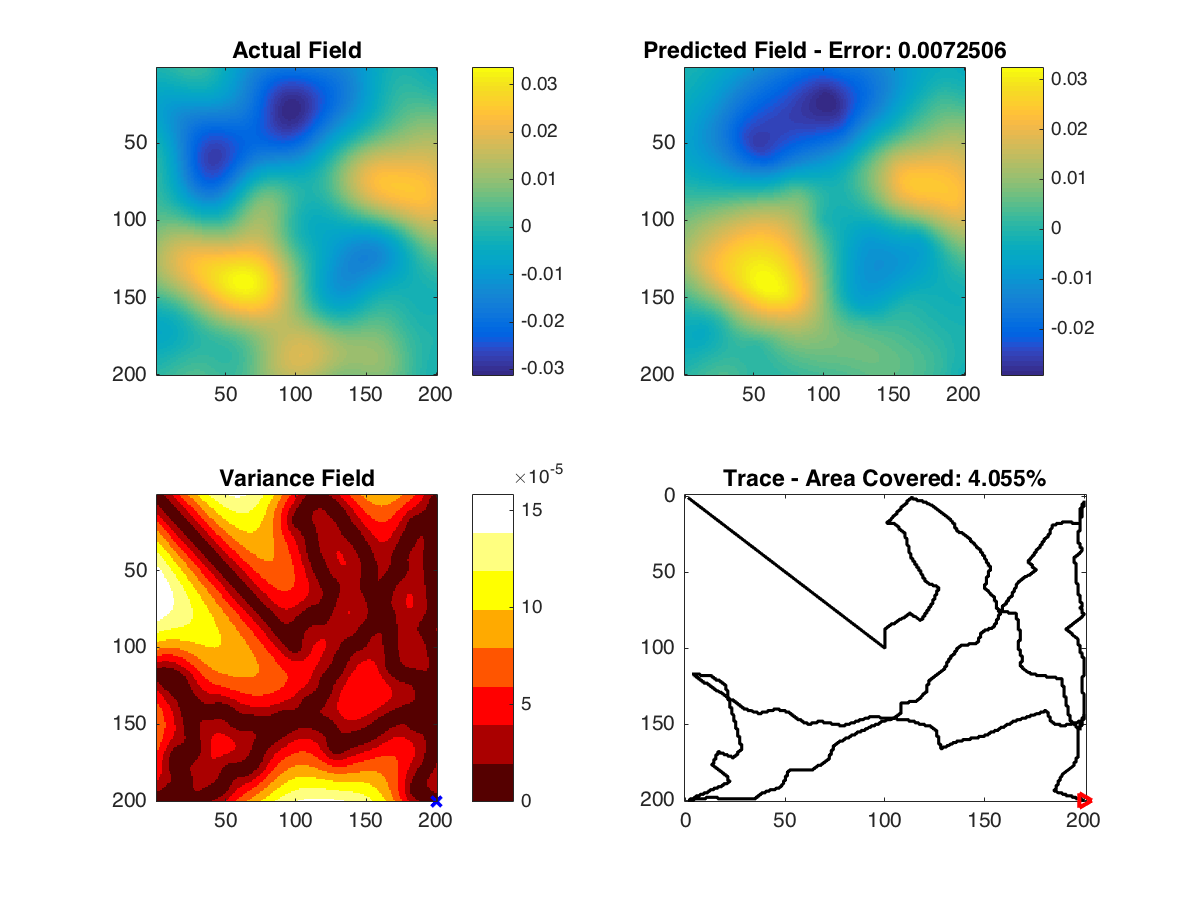
\includegraphics[width=0.8\linewidth]{figures/sim_figures/mc_3_5p_200x200_sf_20_seed_2}
    \captionsetup{skip=0.25\baselineskip}
    \ssp
    \caption{Monte Carlo Path Planning ($N=5$, $M_{mc}=20$). The actual field (top left), predicted field (with error) (top right), variance field (bottom left), and traversed path (bottom right).}
\end{figure}

\begin{figure}[htb!]
    \centering
    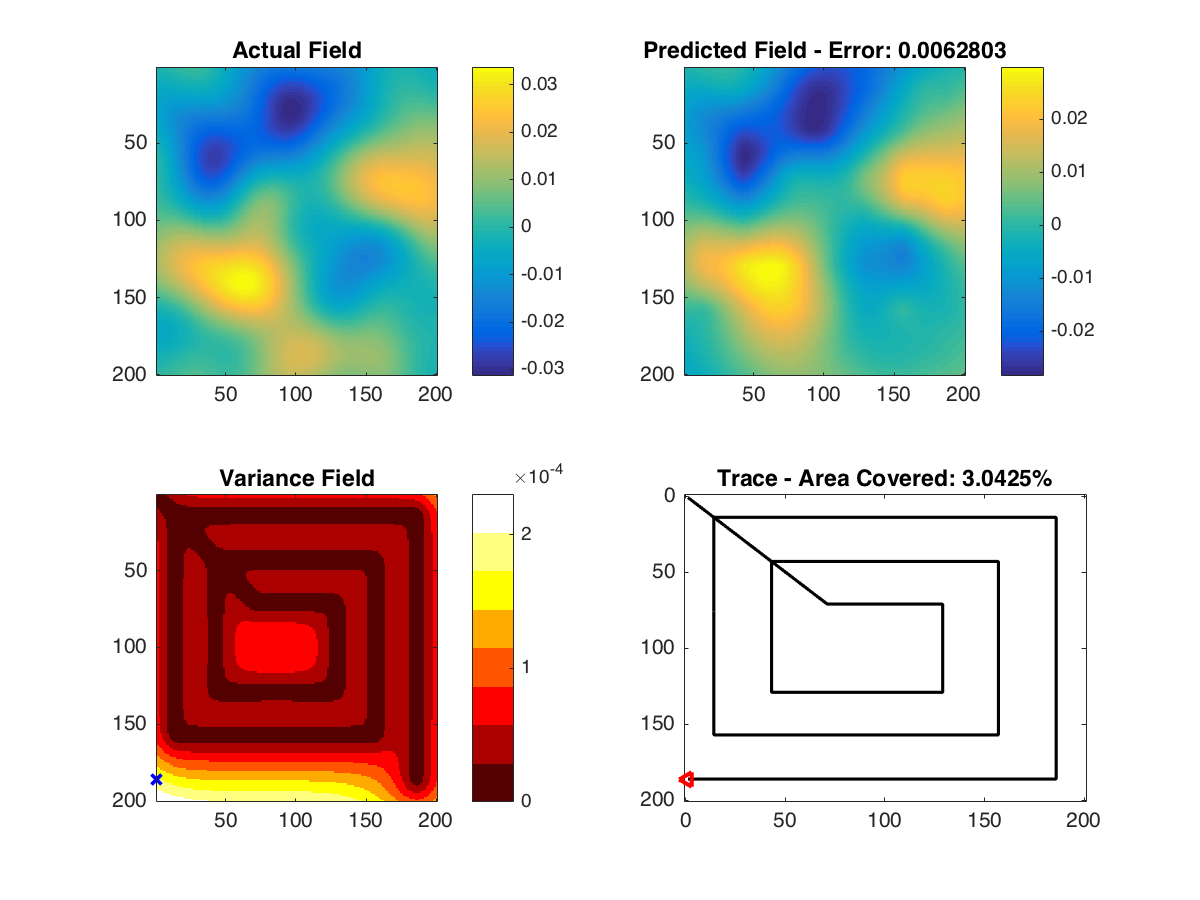
\includegraphics[width=0.8\linewidth]{figures/sim_figures/zz_3_5p_200x200_sf_20_seed_2}
    \captionsetup{skip=0.25\baselineskip}
    \ssp
    \caption{Zig-Zag Method. The actual field (top left), predicted field (with error) (top right), variance field (bottom left), and traversed path (bottom right).}
\end{figure}

\begin{figure}[htb!]
    \centering
    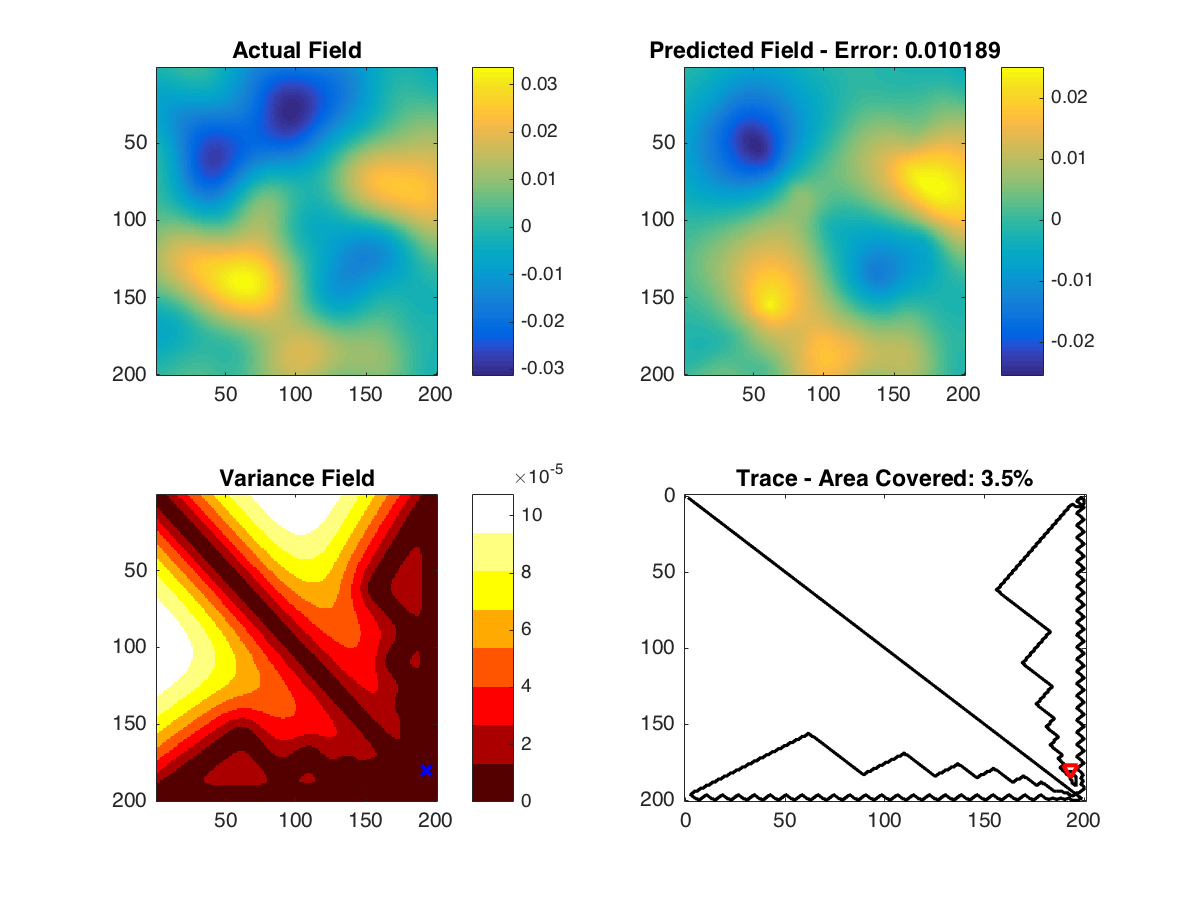
\includegraphics[width=0.8\linewidth]{figures/sim_figures/greedy_3_5p_200x200_sf_20_seed_2}
    \captionsetup{skip=0.25\baselineskip}
    \ssp
    \caption{Greedy Next-Best-View Method. The actual field (top left), predicted field (with error) (top right), variance field (bottom left), and traversed path (bottom right).}
\end{figure}
